\chapter{Design Guidelines for Assistive Devices} \label{sec:chapterDesignGuidelines}

\section{Introduction}

The development of wearable robotic assistive devices requires a deep understanding of human biomechanics. Specifically, the kinematic and kinetic parameters are fundamental for the design stage and the assessment stage of an assistive device. The kinematic parameters describe the human body motion in terms of the angle, velocity, and acceleration of a joint. The kinetic
parameters describe the forces involved in the motion of a joint in terms of torque and mechanical power. The characterization process of these parameters involves reviewing several clinical studies focused on gait analysis. Commonly, the scope of the latter process is limited to the end-application of the assistive device, e.g. assisting healthy adults to walk at the ground level. Therefore, the characterization of the kinematic and kinetic parameters dictates the applicability of the assistive device, in terms of the end-user characteristics. This important step in the design stage of an assistive device is often overlooked. The limitations of the resulting device are then solved by over-sizing it. 

This chapter introduces several techniques to facilitate the extraction of design guidelines for the development of assistive devices through visual representation of the kinematic and kinetic parameters taken from clinical studies on gait analysis. The chapter is organized as follows.

The kinematic and kinetic parameters of the human lower limb during activities of daily living (ADLs) are introduced. These parameters are extracted from clinical studies focused on gait analysis. The underlying difficulties of extracting these parameters from the available literature are discussed. Subsequently, the extracted parameters are categorized and visually represented using different chart designs. Lastly, the benefits of each chart design, in the context of extracting design guidelines for the development of assistive devices, is discussed.

\section{Characterization of Kinematic and Kinetic Parameters for Activities of Daily Living} \label{sec:characterizationKKP}

The kinetic and kinematic parameters of each joint are an important part of the biomechanics of the human body. The kinematic parameters describe the human body motion in terms of the joint angle, velocity, and acceleration. The kinetic
parameters describe the forces causing this motion, e.g. joint torque and power. Motion capture is the most commonly used method to extract these parameters. However, other technologies such as soft strain sensors \cite{mengucc2014wearable}, electrogoniometers \cite{wu2011electromyography}, and inertial measurement units (IMU) have also been used. The process of characterizing these parameters is very important for the development of any wearable robotic device. This allows the intended device to be tailored for a specific application, it being assisting an elder adult or enabling a disabled subject to move. Alternatively, the kinetic and kinematic parameters can be also used to measure the effectiveness and compatibility of an already available assistive device. Measuring the effectiveness of an assistive device in this way is more convenient than calculating the metabolic cost reduction, which involves specialized equipment \cite{panizzolo2016biologically}. 

The kinetic and kinematic parameters can be obtained from gait studies. These studies differ between one another in many aspects, in addition to the technology of choice, such as subjects' gender, age, weight, etc., as well as the setup of the experiments. Therefore, the following subsection describes the process of extracting and processing the kinetic and kinematic parameters from gait studies. As previously mentioned, these parameters are useful design guidelines for wearable robotic devices. The gait studies compiled in the following section cover the main activities of daily living (ADLs), which are: walking, ascending/descending stairs, ascending/descending ramps and chair sitting down/standing up. In the context of studying the human lower limb, the joints of interest are the hip, knee and ankle joints.

\subsection{Gait Analysis Data}

In clinical studies focused on analysing the human gait, parameters regarding the subjects involved and the experiment performed are commonly provided. Regarding the subjects characteristics, information about their age, subject age, weight, height, gender and health condition are included. Similarly, contextual information about the experiment performed such as: loading conditions, plane geometry, and activity of choice is provided. Subjects characteristics are always presented as mean values. In a similar way, measured and calculated data, such as torque and power, are presented in normalized values. The gait cycle is usually normalized using the subjects height, whereas the joint torques are normalized using the subjects weight. The latter is clearly expressed in the units of the reported values, being Nm/kg for the joint torque, and W/kg for the joint mechanical power. Nonetheless, some studies do not follow the same guidelines when reporting the obtained results, or when normalizing the calculated values, preventing the reported information to be compared against other clinical studies \cite{lee2008biomechanics}. 

The diversity on the subjects characteristics difficult the comparison process against similar clinical studies. Due to this, some clinical studies focus on studying a common characteristic among all participants, such as age or health condition. This is the case for the study in \cite{bovi2011multiple}, where the study group is segmented in two age groups. One group included subjects from 22 to 72 years old, meanwhile, the subjects from the other group have ages ranged from 6 to 17 years old. With this segmentation approach, the clinical study can present the results with respect to age range. In some cases where the difference between age groups is very small, the clinical study condense the reported data into a single dataset \cite{lee2008biomechanics}.

The technology of choice to extract the kinematic parameters of the human gait, such as the joint angle, is motion capture. Similarly, the human body kinetics parameters are extracted by measuring the ground reaction forces using force plates. The latter is required to calculate the joint torque and joint power. Therefore, the three most common parameters found in gait analysis studies are the angle, torque, and power of the joint of interest. The gait cycle of the studied activity is usually presented in a chart accompanied with tables to clearly indicates the maximum, minimum and mean values of the gait cycle. The difference between the maximum and minimum values of the kinematic and kinetic parameters of a gait cycle are very important for the characterization process. Commonly, these values are provided in the studies in the form of tables and charts \cite{han2011biomechanical,yali2010biomechanics}, in other cases the complete experiment dataset is included \cite{moore2015elaborate}. The extraction of the parameter of interest is straightforward when the data is presented in a form of a table. Alternatively, when data is provided in the form of charts, the process of extracting it must be done by visual inspection, which inherently add some degree of error to the extracted data \cite{protopapadaki2007hip,riener2002stair,mcintosh2006gait,roebroeck1994biomechanics,mak2003joint}. Likewise, it can be the case for some studies to focus on specific features of the gait cycle, such as maximum and minimum values of each parameter; or to not provide one or more of the parameters of interest (angle, torque or power). Due to all these different scenarios, the process of curating and compiling the data found in clinical studies is very lengthily. The latter motivated the process described in the following section in which the data of several clinical studies is compiled and visually presented to serve as design guidelines for the development of soft robotic applications for human assistance.

\subsection{Extracting Design Guidelines}

The variations of the data from one experiment to another can be reduced by focusing on the range obtained from the difference between the maximum and minimum values of each parameter. This is illustrated in \Cref{fig:HipKKPWalking}, despite the variations between the maximum and minimum values from one experiment to another, the actual range of each parameter is similar among all the experiments. The mean range of motion for the hip joint angle throughout different walking over-ground experiments was found to be 44.63\degree{} (\Cref{fig:HipKKPWalking}). Also, the greatest variation between the mean range value and the range value of each experiment is 18\% of the mean value. The previous calculation can be used to decide design parameters of wearable robotic devices, such as which range of motion should be covered by the device depending on which sector of the population is intended to be assisted. Alternatively, the device can be tailored to cover as much of the population as possible by choosing the maximum and minimum values of the range of motion, out of all the experiments. 
\begin{figure}[htbp]
    \centering
    \begin{subfigure}[b]{0.75\textwidth}
        \centering
        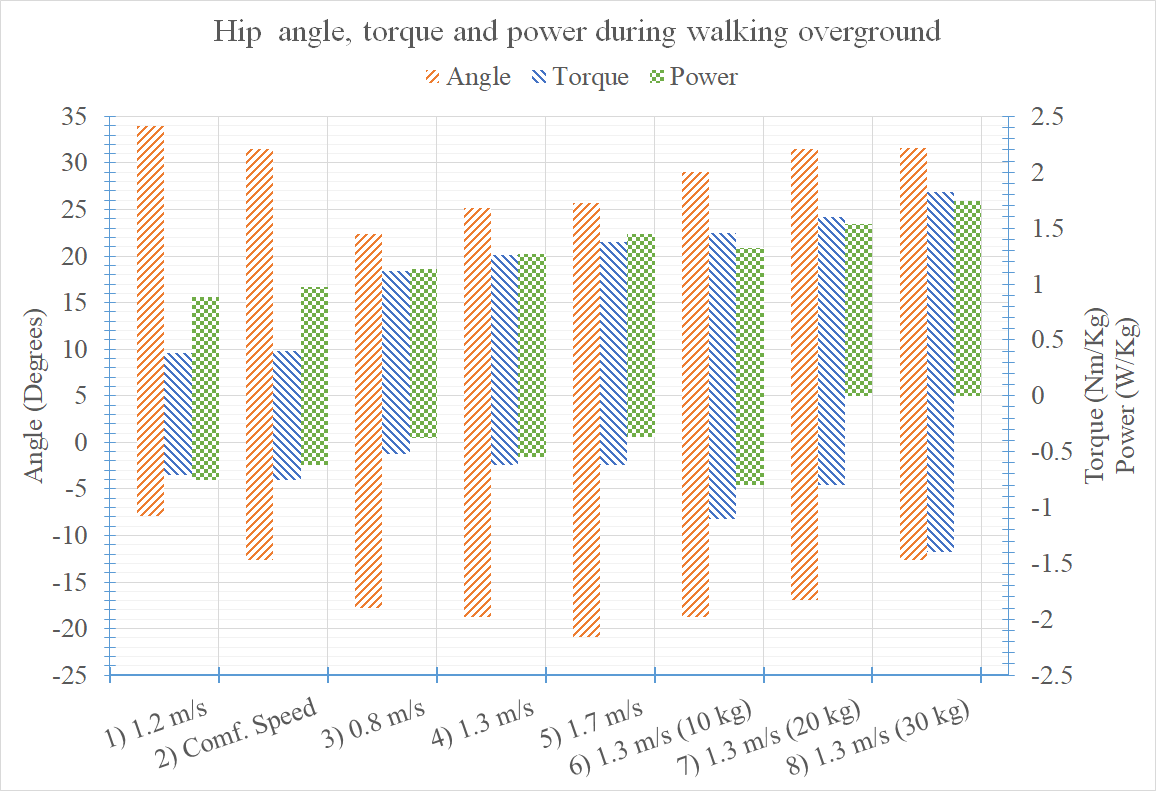
\includegraphics[width=\textwidth]{HipKKPWalkingExcel.png}
        \caption{Hip joint characteristics for walking over ground activities. The weight next to the name of some activities dictates the load carried by the subjects during the experiment \cite{solis2017characterization}. Data collected from: (1) \cite{bovi2011multiple}, (2) \cite{lee2008biomechanics}, (3-8) \cite{han2011biomechanical}. }
        \label{fig:HipKKPWalking}
    \end{subfigure}
    \hfill
    \begin{subfigure}[b]{0.75\textwidth}
        \centering
        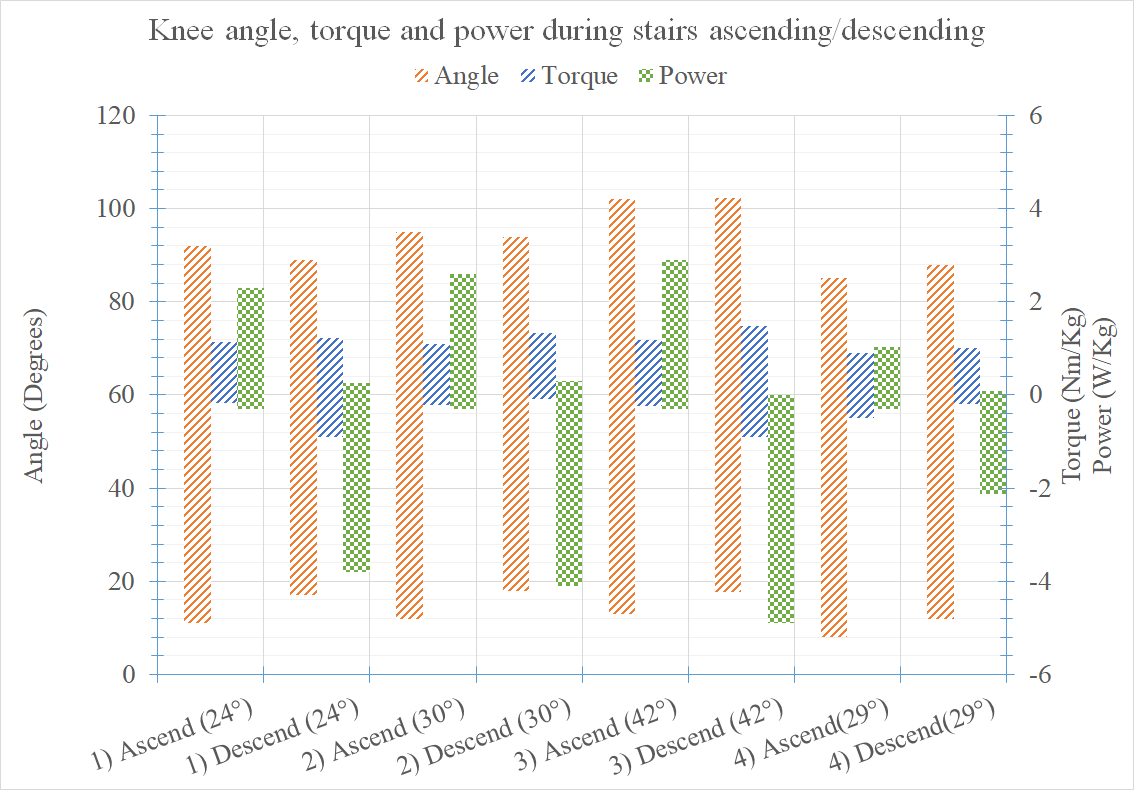
\includegraphics[width=\textwidth]{KneeKKPStairsExcel.png}
        \caption{Knee joint characteristics for several stairs ascending/descending experiments. The number enclosed in brackets represents the stairs slope. Data collected from: (1) \cite{riener2002stair}, (2-4) \cite{reid2007knee}. }
        \label{fig:KneeKKPWalking}
    \end{subfigure}
    \caption[Clustered-stacked bar charts of reviewed gait analyses.]{Clustered-stacked bar charts of reviewed gait analyses \cite{solis2017characterization}. }
    \label{fig:clusteredMain}
\end{figure}

Different design guidelines can be extracted when visually analysing other parameters together. For example, in \Cref{fig:KneeKKPWalking} , the parameters of the knee joint are now compared against many experiments of stairs ascending/descending. Now, the main feature is not the range of motion of the knee, but the characteristics of the torque values. They appeared mirrored, in other words, the torque values required for descending stairs are of similar magnitudes but opposite in direction. Also, the amount required for ascending stairs is generally twice as much as the amount required for descending stairs. The latter illustrates an optimization opportunity. When designing a wearable robotic device for human assistance, the actuator is chosen to satisfy a certain torque range of a particular activity. Without the characterization of the parameters performed, the actuator is most likely to be oversized to comply with the most demanding part of the activity. However, a different approach could be proposed: agonist-antagonist actuators; a technique implemented in several wearable robotic devices which at the same time complies with the actual functionality of the human skeletal muscle system.

Another useful way of extracting design guidelines from the gait analyses is to plot the range of a specific parameter against different ADLs. To the best of the author's knowledge, this approach has only been documented once in \cite{rowe2000knee}, where the range of motion of the knee joint is compiled into a chart for 11 different ADLs. This concept, illustrated in \Cref{fig:HipTorqueRange}, can provide insight of two important design parameters. On the one hand, the actuators meant for this application must be capable of delivering torques in both directions of rotation, i.e. clockwise and anti-clockwise. On the other hand, the selected actuation technology must meet the torque requirements of the activity of interest. \Cref{fig:HipTorqueRange} was constructed using the mean range of the hip joint torque during different activities \cite{bovi2011multiple,lee2008biomechanics,han2011biomechanical,protopapadaki2007hip,riener2002stair,mcintosh2006gait,roebroeck1994biomechanics,mak2003joint}.

\begin{figure}[htbp!]
    \centering
    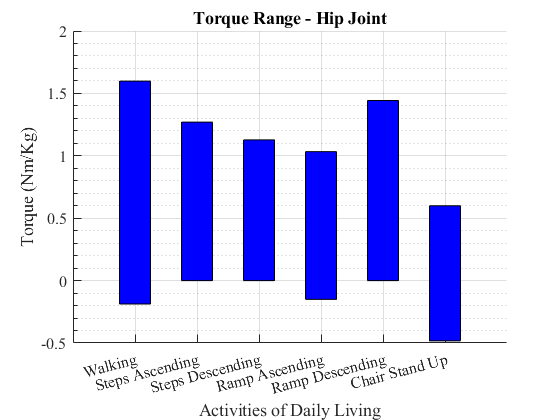
\includegraphics[width=0.8\textwidth]{HipTorqueRange.png}
    \caption[Torque range values during several activities. The values for the maximum and minimum torque are mean values from the data of all the different gait analysis experiments enclosed in one main activity.]{Torque range values during several activities. The values for the maximum and minimum torque are mean values from the data of all the different gait analysis experiments enclosed in one main activity. \cite{bovi2011multiple,lee2008biomechanics,han2011biomechanical,protopapadaki2007hip,riener2002stair,mcintosh2006gait,roebroeck1994biomechanics,mak2003joint,solis2017characterization} }
    \label{fig:HipTorqueRange}
\end{figure}

Another alternative of visual representation of the data can be done by grouping the range of a specific parameter and comparing it with any of the subjects' physical characteristics, e.g. the age range. This is illustrated in \Cref{fig:KneeRangeAge}, where the dependency of the subjects' age with the knee range of motion is evidenced. The colour code used in \Cref{fig:KneeRangeAge}, the age ranges and knee ranges of motion are presented in \Cref{tbl:KneeRangeMotionage}. The chart shown in \Cref{fig:KneeRangeAge} concentrates the data from three different gait analyses, in which six age groups are contained. The approach used in \Cref{fig:KneeRangeAge} is to overlap areas of different colours, each area represents the range of motion of the knee for a specific age range. The area in which several areas intersect can be appreciated due to the enabled transparency property. Nevertheless, the areas where three and two areas are intersected are manually highlighted by a surrounding solid line and dotted line respectively, to improve their visualization. This simple intersection of areas can provide information regarding the required range of motion to be delivered by the wearable robotic device with respect to the aimed population sector.
For example, if a wearable robotic device is aimed to assist the population sector aged from 50 to 70 years old, then a range of motion of the knee joint from 5{\textdegree} to 63{\textdegree} would suffice to meet the requirements. The range of motion is taken from the triple intersection of areas illustrated in \Cref{fig:KneeRangeAge}, which can provide a certain degree of confidence since three different clinical studies are compared. This approach can be used to compare other characteristics, e.g. subject's weight against torque. Summarizing, the overlapping areas approach can provide guidelines to avoid over sizing of wearable robotic devices by analysing the intersection of different areas which ultimately provides a degree of confidence when deciding design parameters.

\begin{table}[htb!]
\caption[Colour code used in \Cref{fig:KneeRangeAge} for each combination of age range and knee range of motion.]{Colour code used in \Cref{fig:KneeRangeAge} for each combination of age range and knee range of motion  \cite{solis2017characterization}.}
\label{tbl:KneeRangeMotionage}
\begin{tabular}{c|c|c|c}
\hline
Colour Code & Knee Range of Motion (\degree{}) & Age Range (Years) & Clinical Study \\
\hline
Red         & 2.2 - 67.4               & 49 - 90           & \cite{rowe2000knee}       \\
Green       & 5 - 66.5                 & 6 - 17            & \cite{bovi2011multiple}        \\
Blue        & 4.5 - 63.5               & 22 - 72           & \cite{bovi2011multiple}           \\
Yellow      & 0 - 69                   & 18 - 30           & \cite{lee2008biomechanics}        \\
Magenta     & 0 - 69                   & 50 - 70           & \cite{lee2008biomechanics}     \\
Cyan        & 8 - 63.6                 & 23 - 27           & \cite{han2011biomechanical}    \\  
\hline
\end{tabular}
\end{table}

\begin{figure}[htb!]
    \centering
    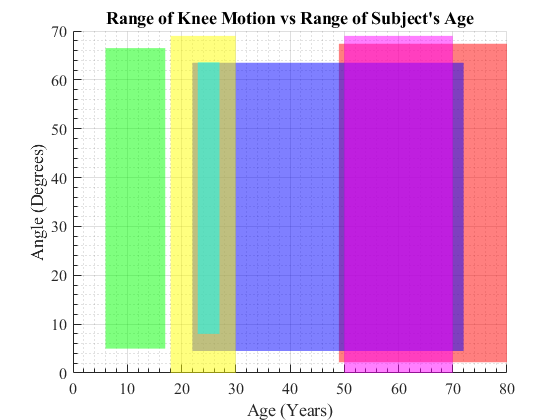
\includegraphics[width=0.7\textwidth]{KneeRangeMotionAge.png}
    \caption[Comparison between subjects' age and the knee range of motion during walking over ground. The areas surrounded by solid lines and dotted lines represent the intersection between three and two areas, respectively. The overlapping squares highlight the great similarity among the range of motion despite subjects' age. The data used to create this chart is presented in \Cref{tbl:KneeRangeMotionage}]{Comparison between subjects' age and the knee range of motion during walking over ground. The areas surrounded by solid lines and dotted lines represent the intersection between three and two areas, respectively. The overlapping squares highlight the great similarity among the range of motion despite subjects' age. The data used to create this chart is presented in \Cref{tbl:KneeRangeMotionage} \cite{solis2017characterization}. }
    \label{fig:KneeRangeAge}
\end{figure}

In this section the process of characterizing the human lower limb kinematics and kinetics parameters during some ADLs is described. The relevant information provided in gait analysis experiments, and the challenges faced when extracting it from the clinical trials, are also explained. Data compiled for the activities of walking, ascending/descending stairs, ascending/descending ramps and chair standing up are presented in the form of clustered stacked bar charts. This type of chart allowed quick and easy detection of similarities between several clinical trials of the same activity. In contrast, the spotted differences, as the ones for the knee torque values during ascending/descending stairs, are indicators for optimization opportunities where instead of using a single actuator to satisfy the torque range, an agonist-antagonist system is more suitable.

The reliability of the data can also be observed using the type chart of overlapping areas with subjects' ranges of age against the knee ranges of motion. In other words, the specific ranges in which the data from different experiments overlaps, gives a measure of consistency which can be used to tailor the developed wearable device coverage. 

The chart style with ranges of motion versus activities, facilitates the choice of the actuator type and dimension (depending on the activities of interest). The styles used to represent the charts are kept as simple as possible while providing useful information about the KKP. However, more complex plotting methods can be used. Finally, a total of 12 charts are produced in Excel\textregistered{} using the compiled data from the gait analyses. In favour of keeping the length of this section adequate, only two out of the 12 charts are included. The remaining charts are in the \Cref{appendixA}.

\section{Summary}

The characterization of the kinetic and kinematic parameters of the hip, knee and ankle joints is performed by reviewing many clinical trials about gait analysis of the lower limb. The collected data can be used as design guidelines when developing robotic devices targeted for human assistance. Therefore, many visualization techniques are proposed and analysed in this context. The latter work resulted in a published conference paper (\Cref{sec:characterizationKKP}). In summary, the main findings of this chapter are as follows:

The visual approach presented in \Cref{fig:clusteredMain} makes use of clustered-stacked bars. Visualizing the parameters of angle, torque, and power, against different variations of a specific activity in this way allows the extraction of design guidelines in terms of the intended coverage of the assistive device. In other words, decisions to prioritize specific walking speed, to mention one factor, can be made depending on the en application of the assistive device. The visual approach presented in \Cref{fig:HipTorqueRange} makes use of stacked bars to illustrate the full range of each parameter. This is useful when deciding the capacity of the actuator to be implemented, specially when implementing the antagonist-agonist functionality of a muscle group. In contrast, the information in these charts can also be used to tailor half of the full range of motion of the joint to reduce costs associated with actuators working in pairs. Lastly, the visual approach presented in \Cref{fig:KneeRangeAge} makes use of overlapping square shapes. These shapes represent ranges of two variables of two variables of interest. In the example provided in this chapter, the range of motion of the knee is compared against the subjects age. The information in this chart allows the comparison of physiological aspects of the subject against the joint range of motion. This allows the intended assistive device to be fine tune to a specific target group. In other words, this allows the properly selection of the actuator to be implemented in the assistive device.

